
\onecolumn
\chapter{Office 365 の設定 その1}
\label{chap:O365設定1}


第\ref{chap:O365設定1}章では、Windows デバイスの展開に必要な Office 365 の設定に監視て解説いたします。Office 365 を安心・安全にお使いいただくための設定については、第\ref{chap:O365設定1}章で解説いたしますのでそちらをご参照ください。
  
%%%%%%%%%%%%%%%%%%%%%%%%%%%%%%%%%%%%%%%%%%%%%%%%%%%%%%%%%%%%%%%%%%%%%%%%%%%%%%%%
\begin{figure*}[htbp]
    \begin{minipage}{1.0\textwidth}
        \section{Microsoft 365 管理センターにアクセスする}
        \label{sec:M365管理センター}
    \end{minipage}
\end{figure*}
%%%%%%%%%%%%%%%%%%%%%%%%%%%%%%%%%%%%%%%%%%%%%%%%%%%%%%%%%%%%%%%%%%%%%%%%%%%%%%%%

\begin{figure*}[h]
    \begin{minipage}{0.6\textwidth}
        \vspace{-1.5cm}
        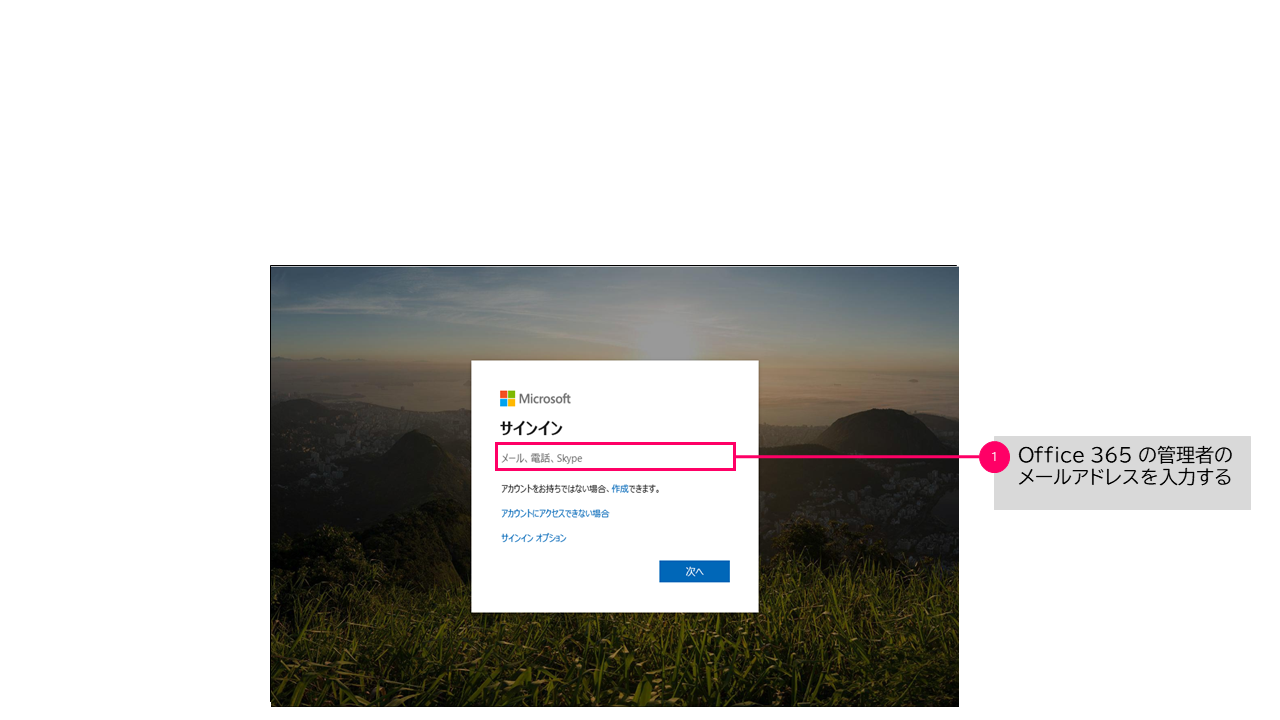
\includegraphics[width=10cm]{figures/M365_setting1-00.png}
    \end{minipage}
    \begin{minipage}{0.4\textwidth}
        1. Webブラウザから、\url{<https://portal.office.com/>} にアクセスします。サインインの画面が表示されたら、Office 365 の管理者のメールアドレスとパスワードでログインします。
    \end{minipage}
\end{figure*}

\begin{figure*}[h]
    \begin{minipage}{0.6\textwidth}
        \vspace{-1.5cm}
        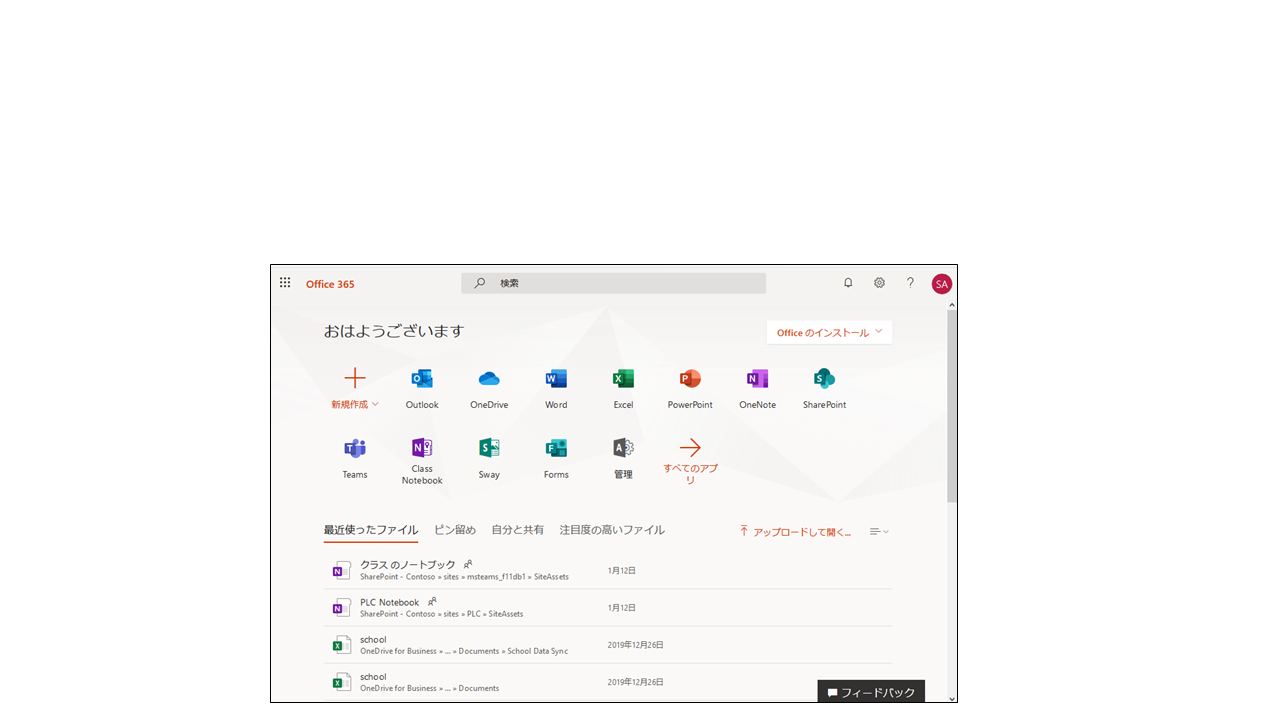
\includegraphics[width=10cm]{figures/M365_setting1-01.png}
    \end{minipage}
    \begin{minipage}{0.4\textwidth}
        2. ログインが完了すると Microsoft 365 の管理画面が表示されます。
    \end{minipage}
\end{figure*}

%%%%%%%%%%%%%%%%%%%%%%%%%%%%%%%%%%%%%%%%%%%%%%%%%%%%%%%%%%%%%%%%%%%%%%%%%%%%%%%%
\begin{figure*}[h]
    \begin{minipage}{1.0\textwidth}
        \section{メールドメインの追加}
        \label{sec:メールドメインの追加}
    \end{minipage}
\end{figure*}
%%%%%%%%%%%%%%%%%%%%%%%%%%%%%%%%%%%%%%%%%%%%%%%%%%%%%%%%%%%%%%%%%%%%%%%%%%%%%%%%

\begin{figure*}[h]
    \begin{minipage}{0.6\textwidth}
        \vspace{-1.5cm}
        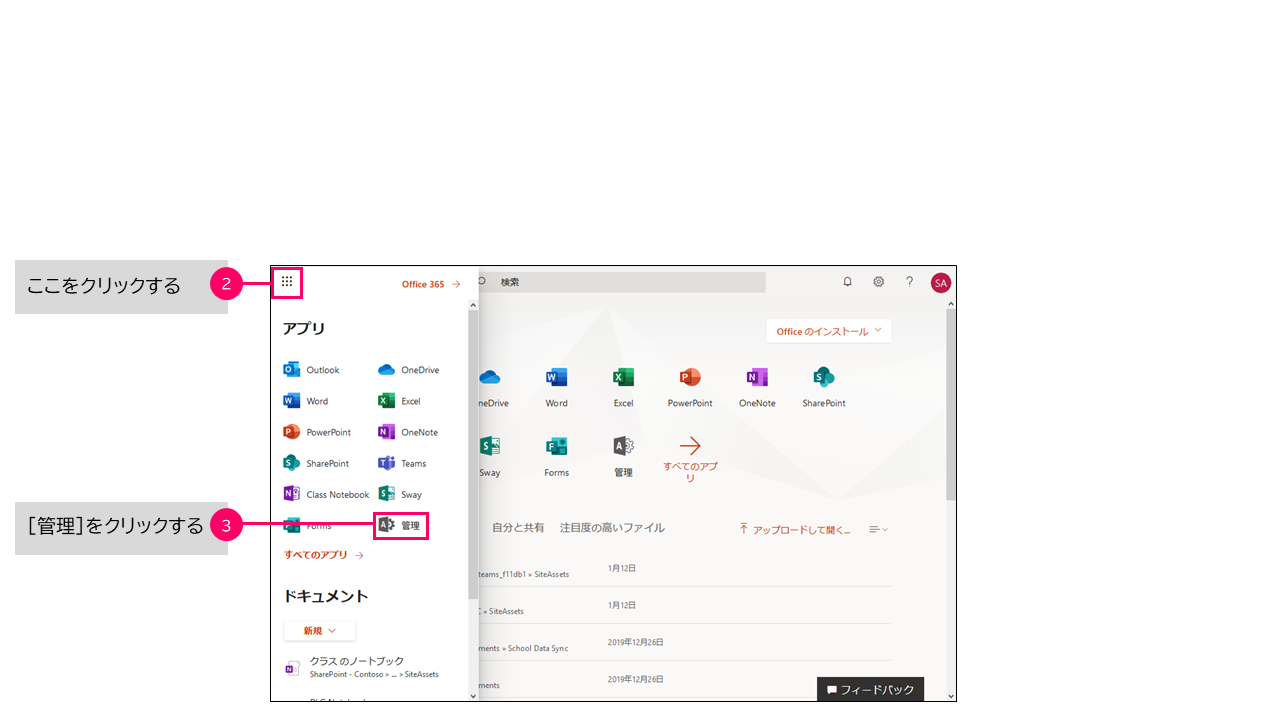
\includegraphics[width=10cm]{figures/M365_setting1-02.png}
    \end{minipage}
    \begin{minipage}{0.4\textwidth}
        3. 画面右上のメニューアイコンをクリックしてください。\\
        4. \textbf{【管理】}をクリックしてください。
    \end{minipage}
\end{figure*}

\begin{figure*}[h]
    \begin{minipage}{0.6\textwidth}
        \vspace{-2cm}
        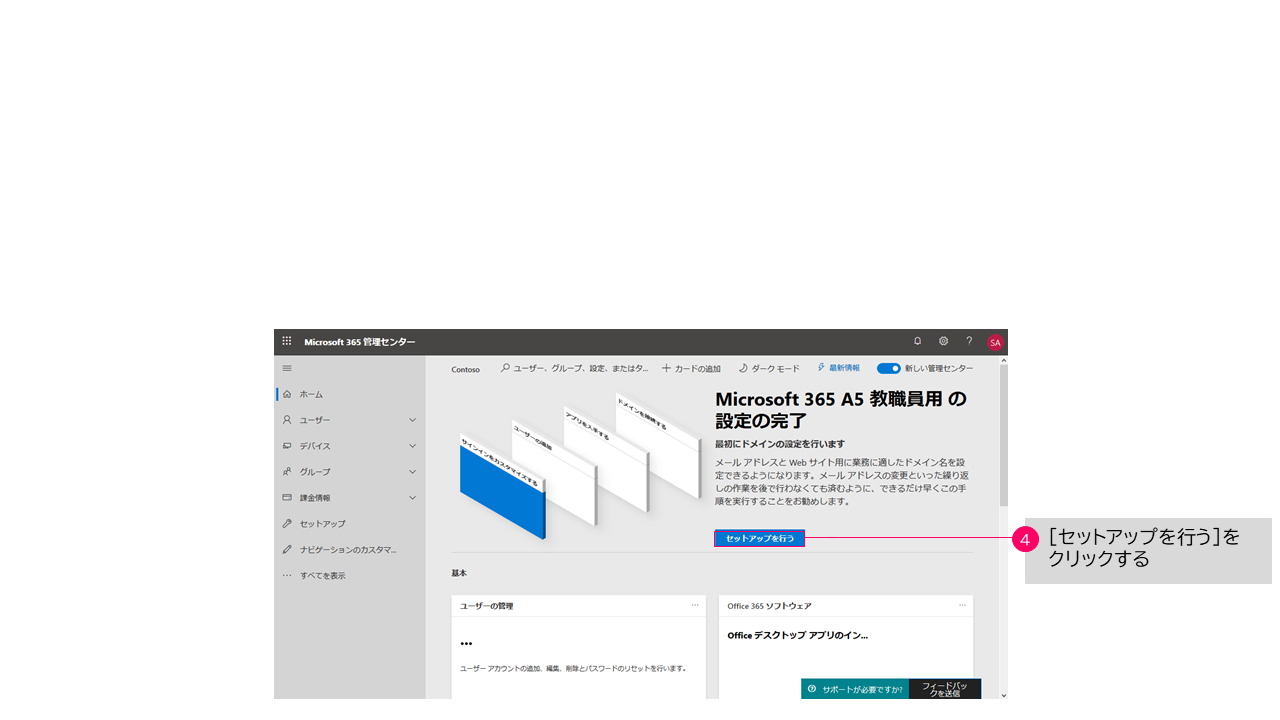
\includegraphics[width=10cm]{figures/M365_setting1-03.png}
    \end{minipage}
    \begin{minipage}{0.4\textwidth}
        5. \textbf{【セットアップを行う】}をクリックしてください。
    \end{minipage}
\end{figure*}

\begin{figure*}[h]
    \begin{minipage}{0.6\textwidth}
        \vspace{-1.5cm}
        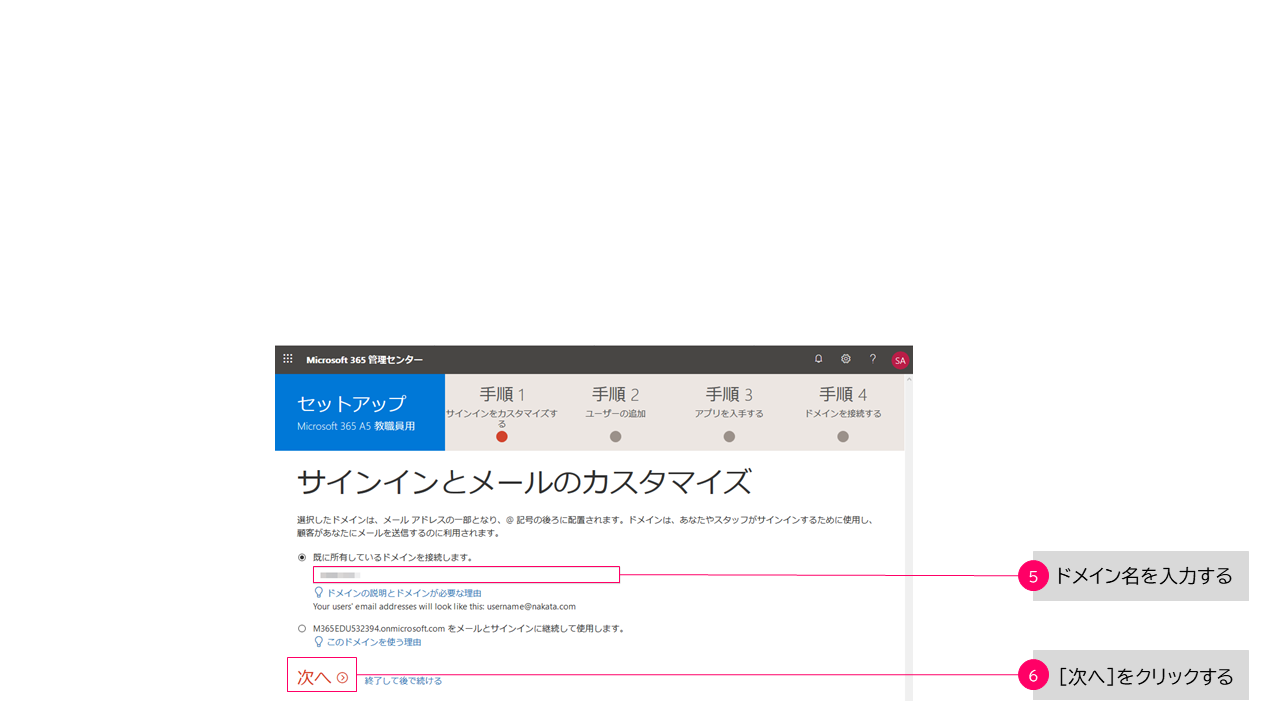
\includegraphics[width=10cm]{figures/M365_setting1-04.png}
    \end{minipage}
    \begin{minipage}{0.4\textwidth}
        6. \textbf{「サインインとメールのカスタマイズ」}の画面が表示されたら、所有しているメールドメインを入力し、\textbf{【次へ】}をクリックしてくださだい。
    \end{minipage}
\end{figure*}

\begin{figure*}[h]
    \begin{minipage}{0.6\textwidth}
        \vspace{-1cm}\hspace{-0.5cm}
        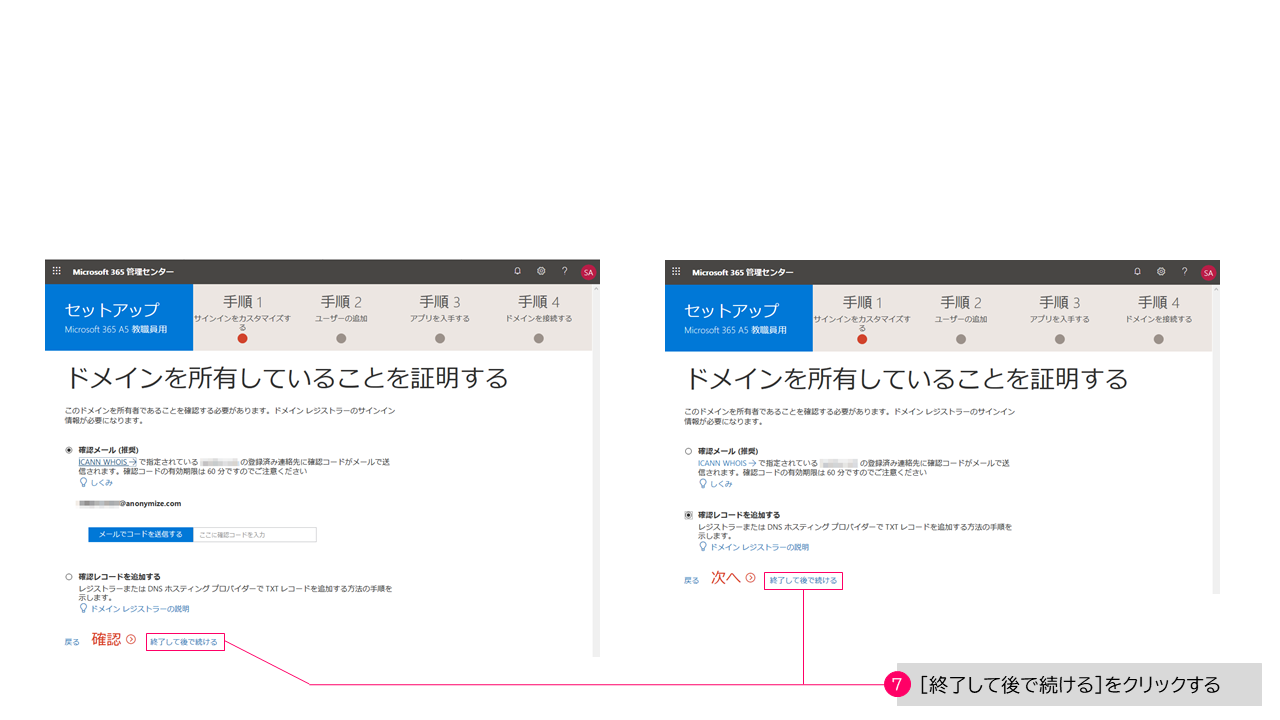
\includegraphics[width=10cm]{figures/M365_setting1-05.png}
    \end{minipage}
    \begin{minipage}{0.4\textwidth}
        7. \textbf{ドメインを所有していることを証明する】}の画面が表示されます。ドメインの所有権の証明する方法としては (1) ICANN WHOS \url{<https://lookup.icann.org/>} に登録しているメールアドレスに確認コードを送り、その確認コードで証明する方法と (2) DNSにTXTレコードを追加し証明する方法の2種類があります。どちらかの方法でドメインの所有権を証明しましたら、\textbf{【終了して後を続ける】}をクリックしてください。
    \end{minipage}
\end{figure*}

%%%%%%%%%%%%%%%%%%%%%%%%%%%%%%%%%%%%%%%%%%%%%%%%%%%%%%%%%%%%%%%%%%%%%%%%%%%%%%%%
\begin{figure*}[h]
    \begin{minipage}{1.0\textwidth}
        \section{ユーザー登録}
        \label{sec:ユーザー登録}
    \end{minipage}
\end{figure*}
%%%%%%%%%%%%%%%%%%%%%%%%%%%%%%%%%%%%%%%%%%%%%%%%%%%%%%%%%%%%%%%%%%%%%%%%%%%%%%%%

\begin{figure*}[h]
    \begin{minipage}{1.0\textwidth}
         Office 365 では、Microsoft 365 管理センターより GUI(Graphical User Interface) で1人1人登録する方法がありますが、ここでは CSVファイルを使用して一括登録する方法を解説します。
    \end{minipage}
\end{figure*}

%%%%%%%%%%%%%%%%%%%%%%%%%%%%%%%%%%%%%%%%%%%%%%%%%%%%%%%%%%%%%%%%%%%%%%%%%%%%%%%%
\begin{figure*}[h]
    \begin{minipage}{1.0\textwidth}
        \subsection{ユーザー一括登録用のCSVファイルの準備}
    \end{minipage}
\end{figure*}
%%%%%%%%%%%%%%%%%%%%%%%%%%%%%%%%%%%%%%%%%%%%%%%%%%%%%%%%%%%%%%%%%%%%%%%%%%%%%%%%